\chapter{Hintergrundwissen}%
\label{cha:Hintergrundwissen}

\section{Konvexe Funktionen}%
\label{sec:Konvexe Funktionen}

\begin{definition}
\label{thm:konvexmenge}
	Eine Menge $X \subseteq \R^{n}$ heißt \underline{konvex} , wenn gilt
	\[
		\forall x,y \in X, \forall c \in [0,1] \colon 
		cx + (1-c)y \in X
	.\] 
\end{definition}

\begin{beispiel}
\label{thm:bspkonvexmenge}
Einige Beispiele

\begin{figure}[ht!]
	\begin{center}
		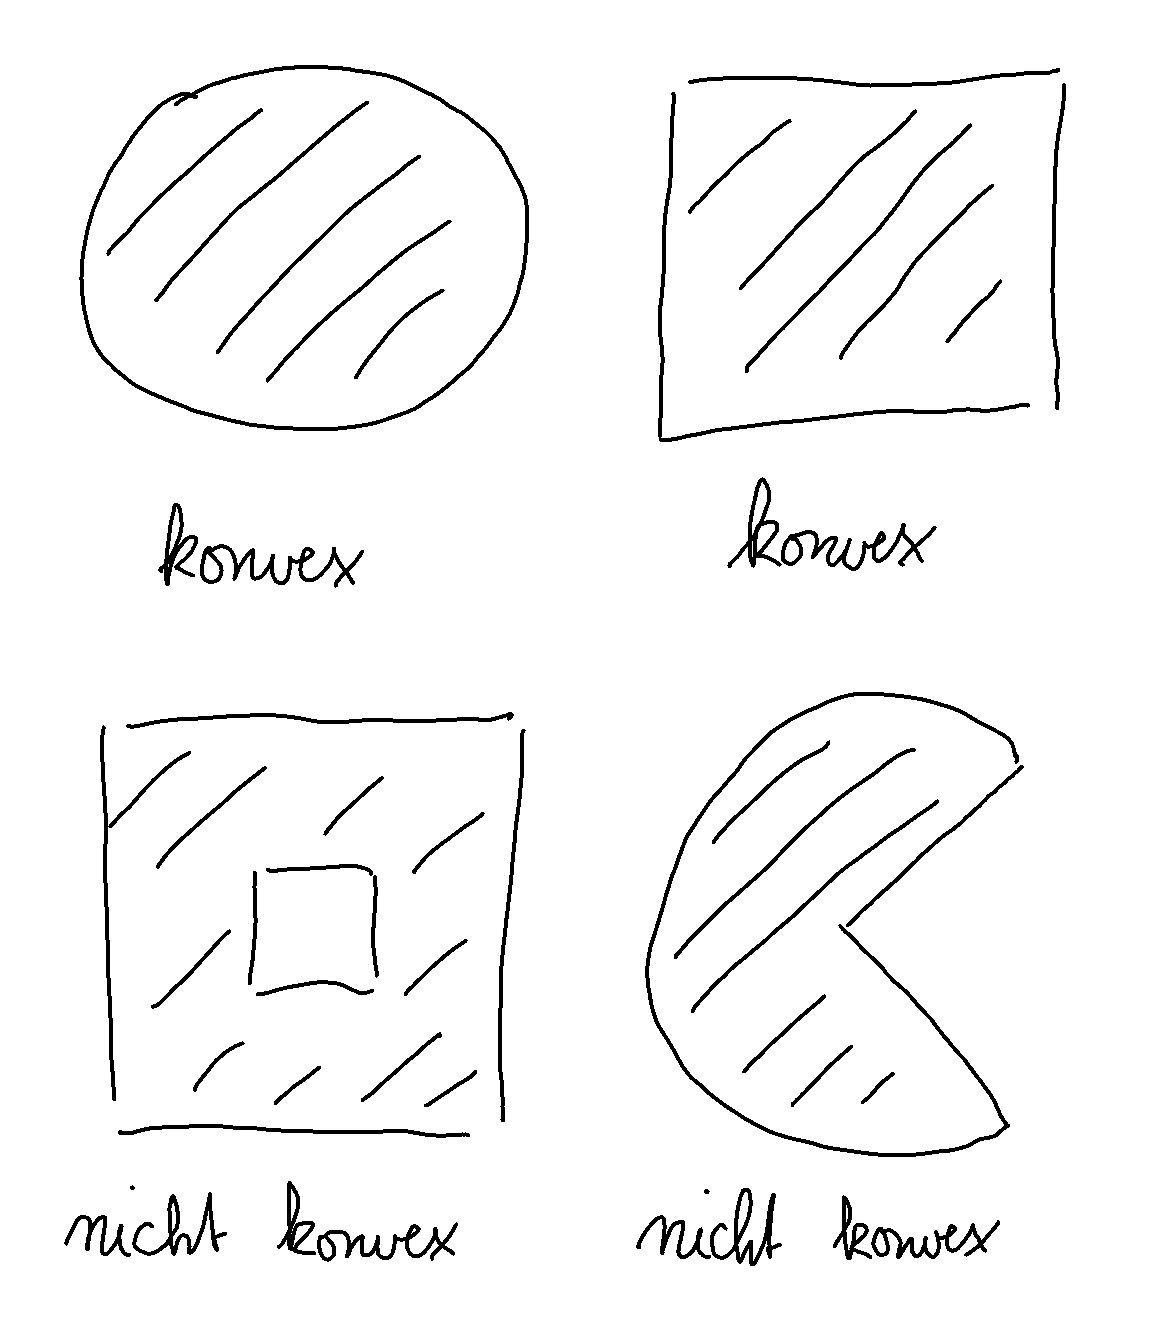
\includegraphics[width=0.5\textwidth]{pics/2.png}
	\end{center}
	\caption{Beispiele konvexer und nicht-konvexer Mengen}
	\label{fig:konvexemengen}
\end{figure}

\end{beispiel}

\begin{definition}
\label{thm:konvexfunktion}
	Sei $X \subseteq \R^{n}$ konvex. Dann heißt $f:X \rightarrow \R$
	\begin{enumerate}[label=\alph{enumi})]
		\item \underline{konvex} (auf $X$), wenn gilt
			\[
				\forall x,y \in X, \forall c \in [0,1] \colon f(cx + (1-c)y) \leq cf(x) + (1-c)f(y)
			.\] 
		\item \underline{strikt konvex} (auf $X$), wenn gilt
			\[
				\forall x,y \in X, x \neq y, \forall c \in (0,1) \colon f(cx + (1-c)y) < cf(x) + (1-c)f(y)
			.\] 
		\item \underline{gleichmäßig konvex} (auf $X$), wenn es ein $\mu>0$ gibt mit
			\[
				\forall x,y \in X, \forall c \in [0,1] \colon f(cx+ (1-c)y) \leq cf(x) + (1-c)f(y) - \mu c(1-c) \norm{x-y}^{2}
			.\] 
			\begin{figure}[ht!]
			\begin{center}
				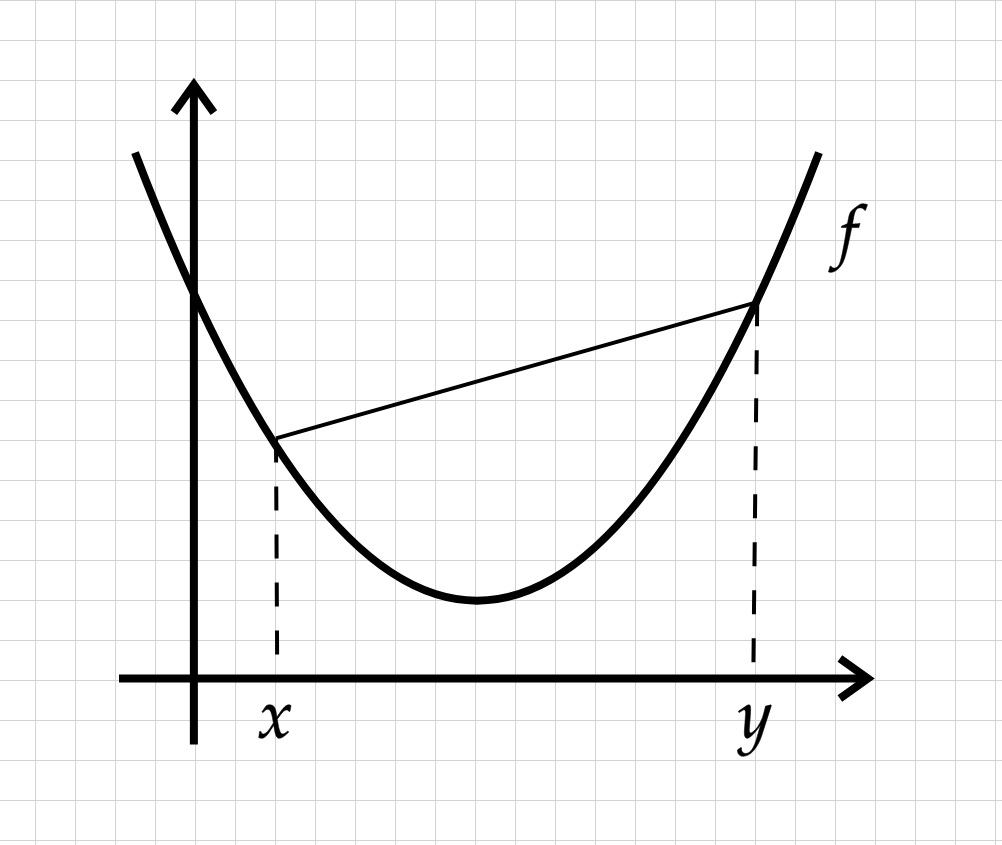
\includegraphics[width=0.4\textwidth]{pics/texplot1.png} 
				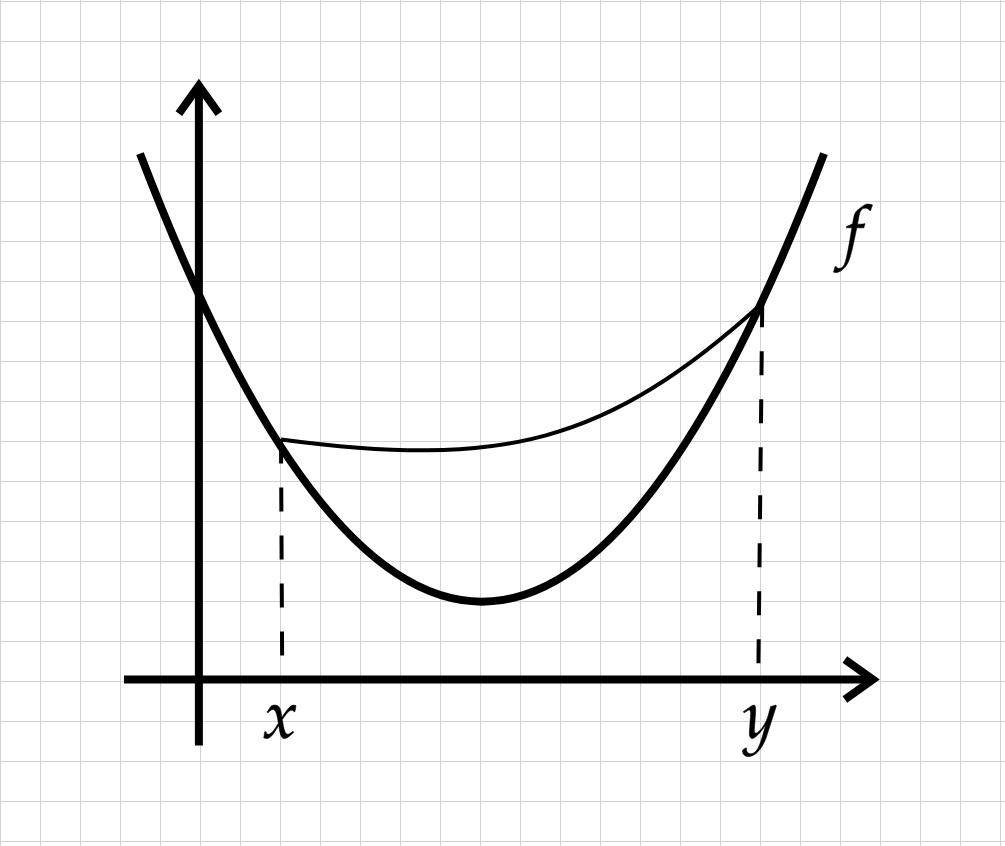
\includegraphics[width=0.4\textwidth]{pics/texplot2.png}
			\end{center}
			\caption{links: konvexe Funktion, rechts: glm. konvexe Funktion}
			\label{fig:glmkonvexefunktion}
			\end{figure}
			
	\end{enumerate}
	Es gilt außerdem
	\[
	f \text{ glm. konvex} \implies f \text{ strikt konvex} \implies f \text{ konvex}
	.\] 
\end{definition}

\begin{beispiel}
\label{thm:bspkonvexfunktion1}

Einige Beispiele für konvexe Funktionen:
\begin{enumerate}[label=\alph{enumi})]
	\item $f$ konvex, aber nicht strikt konvex : $f(x)=c, f(x)=ax$
	\item $f$ strikt konvex, aber nicht glm. konvex : $f(x)=e^{x}, f(x)= x^{4}$
\end{enumerate}
\end{beispiel}

\begin{beispiel}
\label{thm:bspkonvexfunktion2}
Sei $f\colon \R^{n} \rightarrow \R$ mit 
\[
f(x) = \frac{1}{2}x^{T}Qx + c^{T}x+ \gamma
,\]

wobei $Q=Q^{T}$ (sonst $\tilde{Q}= \frac{1}{2}(Q+Q^{T})$). Dann gilt
\[
	cf(x)+(1-c)f(y) = f(cx+(1-c)y) + c(1-c)(x-y)^{T}Q(x-y)
\] 
und damit sieht man 
\begin{align*}
	f \text{ konvex auf } \R^{n} &\iff Q \text{ pos. semidef.} \\
	f \text{ strikt konvex auf } \R^{n} &\iff Q \text{ pos. def.} \iff f \text{ glm. konvex} \\
	Q \text{ pos. def. } &\implies c(1-c)(x-y)^{T}Q(x-y) \geq c(1-c)\norm{x-y} ^2 \underbrace{\lambda_{\min}(Q)}_{=:\mu} 
\end{align*}
\end{beispiel}

\begin{satz}
\label{thm:konvexcharakterisierung}
Sei $X \subseteq \R^{n}$ konvex und $f \colon X \rightarrow \R$ stetig differenzierbar. Dann gelten:
\begin{enumerate}[label=\alph{enumi})]
	\item $f$ konvex $\iff \forall x,y \in X \colon f(y) \geq f(x) + \nabla f(x)^{T}(y-x)$
	\item $f$ strikt konvex $\iff \forall x,y \in X, x \neq y \colon f(y) > f(x) + \nabla f(x)^{T}(y-x)$
	\item $f$ glm. konvex $\iff$ 
		\[
		\exists \mu > 0 \forall x,y \in X \colon f(y) \geq f(x) + \nabla f(x)^{T}(y-x) + \mu \norm{y-x} ^2
		.\]
\end{enumerate}
\end{satz}

\begin{proof}
\label{thm:konvexcharakterisierungbeweis}

\begin{itemize}[label=]
	Wir beweisen zunächst Fall (c), da der Rest schnell aus diesem Fall folgt.
	\item (c)
		\begin{itemize}[label=]
			\item "$\Leftarrow$"

 		Sei $\mu>0$, sodass 
		\[
		\forall x,y \in X \colon f(y)\geq f(x) + \nabla f(x)^{T}(y-x) + \mu \norm{x-y} ^2
		\] 
		erfüllt ist.

Seien $x,y \in X$ und $c \in [0,1]$ und $z = cx +(1-c)y$
\begin{align*}
	\implies & f(x) \geq f(z) + \nabla f(z)^{T}(x-z) + \mu \norm{x-z} ^2 \\
			 &f(y) \geq f(z) + \nabla f(z)^{T}(y-z) + \mu \norm{y-z} ^2 \\
	\overset{\text{Add.}}{\implies} &cf(x) + (1-c)f(y) \geq f(z) + \nabla f(z)^{T}[c(x-z) + (1-c)(y-z)] +  \underbrace{\mu c \norm{x-z} ^2 + \mu(1-c) \norm{y-z} ^2}_{2\mu c(1-c) \norm{x-y} ^2}  \\
	\implies &f \text{ glm. konvex.}
\end{align*}

\item "$\Rightarrow$"

	Sei $f$ glm. Konvex, d.h. $\exists \mu > 0, \forall x,y \in X, \forall c \in [0,1]$, sodass gilt
	\[
	f(cx+(1-c)y) \leq c(fx) + (1-c)f(y) - \mu  c(1-c) \norm{y-x} ^2
	.\] 
\begin{align*}
	\implies &f f(y+ c(x-y)) - f(y) \leq f(x) - f(y) - \mu (1-c)\norm{x-y}^2 \\
	\overset{c \downarrow 0}{\implies} & \nabla f(y)^{T}(x-y) \leq f(x) - f(y) - \mu \norm{x-y} ^2
\end{align*}
		\end{itemize}

	\item (a)

		analog zu (c) mit $\mu = 0$.

	\item (b)

		\begin{itemize}[label=]
			\item "$\Leftarrow$"

 $\mu=0$, $>$ statt $\geq$, $x \neq y$, $c \in(0,1)$ analog zu (c)

 \item "$\Rightarrow$"

 geht nicht völlig analog zu (c) wegen Grenzübergang $c \downarrow 0$.

 Sei $f$ strikt konvex und $x\neq y$, $x,y \in X$. Dann gilt durch (a):
\[
	f(z) \geq f(x) + \nabla f(x)^{T}(z-x)
\] 
$  \text{mit }z=\frac{1}{2}x + \frac{1}{2}y \text{ und } f(z) < \frac{1}{2}f(x) + \frac{1}{2}f(y)$ 

Und damit folgt
\[
	f(y) > f(x) + \nabla f(x)^{T}(x-y)
.\] 
	\end{itemize}
\end{itemize}

\end{proof}

\section{Verallgemeinerungen von Konvexität}%
\label{sec:Verallgemeinerungen von Konvexität}

\begin{definition}
\label{thm:pseudokonvexität}
	Sei $X \subseteq \R^{n}$ off und $f \colon X \rightarrow \R $ differenzierbar. Dann heißt $f$ \underline{pseudokonvex} auf $X$ genau dann, wenn gilt 
	\[
		\forall x,y \in X \colon \underbrace{\nabla f(x)^{T}(y-x)}_{=f'(x; y-x)} \geq 0 \implies f(y) \geq f(x)
	.\] 
Es gilt außerdem
\begin{align*}
	f \text{ konvex + diff'bar } & \implies f(y) \geq f(x) + \nabla f(x)^{T}(y-x) \forall x,y \in X \\
								 & \iff f(y) - f(x) \geq \nabla f(x)^{T}(y-x) \forall x,y \in X \\
								 &\implies f \text{ pseudokonvex}
\end{align*}
\end{definition}


\begin{beispiel}
\label{thm:bsppseudokonvex}
Eine Funktion $f$, die pseudokonvex, aber nicht konvex ist : $f(x) = x^{3} + x$. Hier reicht es nicht aus $f(x)=x^{3}$ zu nehmen, da diese Funktion nicht pseudokonvex ist.
\end{beispiel}

\begin{satz}
\label{thm:stationäresatz}
	Sei $X \subseteq \R^{n}$ konvex und $f \colon X \rightarrow \R $ pseudokonvex. Dann ist ${x}^{*} \in X$ genau dann ein globales Minimum von $f$ auf $X$, wenn ${x}^{*}$ ein \underline{stationärer Punkt} ist, d.h
	\[
		\forall x \in X \colon \nabla f({x}^{*})^{T}(x-{x}^{*}) \geq 0
	.\]
	[Spezialfall : $X = \R^{n}$, ${x}^{*}$ stationär $\iff \nabla f(x) = 0$]
\end{satz}

\begin{proof}\enter
\label{thm:stationäresatzbeweis}
\begin{itemize}[label=]
	\item "$\Rightarrow$"

		Sei ${x}^{*}$ ein (lokales oder globales) Minimum von $f$ auf der konvexen Menge $X$.

Sei $x \in X$ beliebig, dann
\begin{align*}
	\implies &\forall c \in [0,1] \colon x^{0}+c(x-{x}^{*}) \in X \\
	\implies &\nabla f({x}^{*})^{T}(x-{x}^{*}) = \lim\limits_{c\downarrow 0}f({x}^{*}+c(x-{x}^{*}))-f({x}^{*}) \geq 0
\end{align*}

\item "$\Leftarrow$"

	Sei ${x}^{*}$ ein stationärer Punkt, d.h. es gelte
\begin{align*}
	&\nabla f({x}^{*})^{T}(x-{x}^{*}) \geq 0 \forall x \in X \\
	\overset{f \text{ pseudokonvex}}{\implies} &\forall x \in X \colon f(x) \geq f({x}^{*})
\end{align*}
,d.h. ${x}^{*}$ ist globales Minimum.
\end{itemize}
\end{proof}

\begin{definition}
\label{thm:quasikonvex}
Sei $X \subseteq \R^{n}$ konvex. Dann heißt $f \colon X \rightarrow \R $ \underline{quasikonvex} (auf $X$), wenn gilt
\[
	\forall x,y \in X \forall c \in [0,1] \colon f(cx + (1-c)y) \leq \max\limits_{}\left\{ f(x), f(y) \right\} 
.\] 

Außerdem gilt
\[
f \text{ konvex } \implies f \text{ quasikonvex }
.\] 
\end{definition}

\begin{beispiel}\enter
\label{thm:quasikonvexbsp}
\begin{itemize}
	\item Jede monoton wachsende/fallende Funktion $f \colon \R \rightarrow \R $ is quasikonvex
	\item $f(x) = x^{3}$ is quasikonvex, aber weder konvex noch pseudokonvex
	\item quasikonvexe Funktionen können lokale (aber nicht globale) Minima haben
\end{itemize}
\begin{figure}[ht!]
\begin{center}
	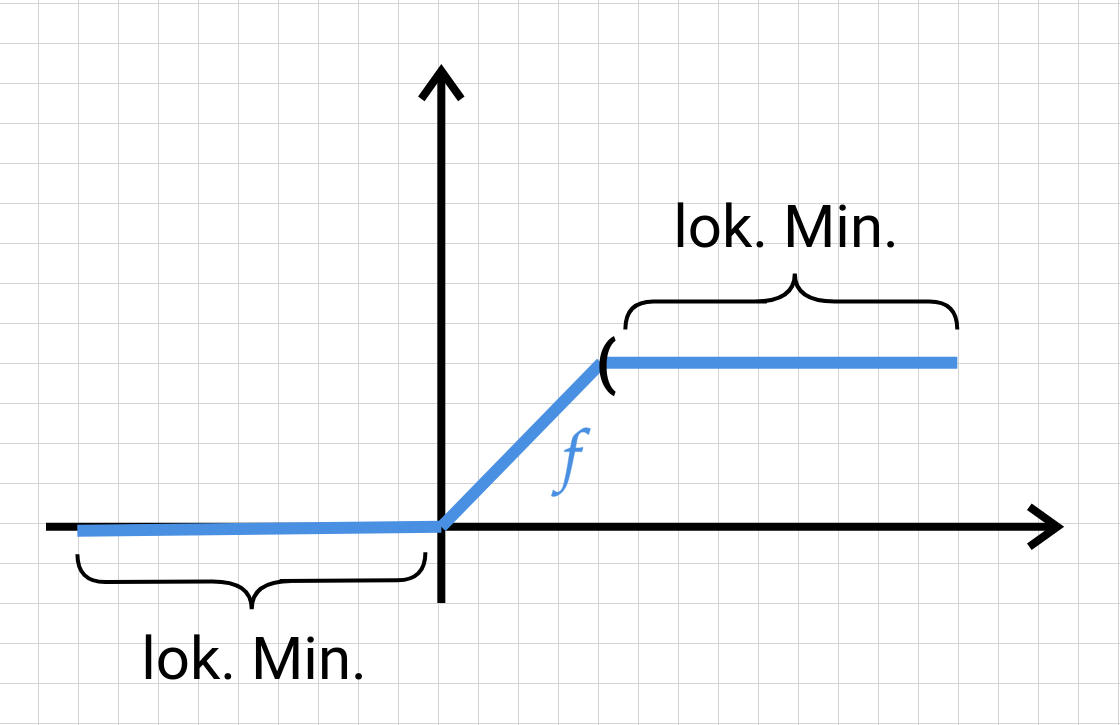
\includegraphics[width=0.5\textwidth]{pics/texplot3.png}
\end{center}
\caption{Quasikonvexe Funktion mit lokalem Minimum, dass zugleich globales Maximum ist}
\label{fig:quasikonvexeFunktion}
\end{figure}

\end{beispiel}

\begin{lemma}
\label{thm:quasikonvexlemma}
	Sei $X \subseteq \R^{n}$ konvex. Dann ist $f \colon X \rightarrow \R $ quasikonvex $\iff$
	$\forall c \in \R$ ist die Levelmenge 
	\[
	L_{c}(f) := \left\{ x \in X | f(x) \leq c \right\} 
	\] konvex.
\end{lemma}

\begin{proof}
\label{thm:quasikonvexlemmabeweis}
	Definitionen + Nachrechnen
\end{proof}

\begin{satz}
\label{thm:pseudoundquasikonvexität}
	Sei $X \subseteq \R^{n}$ offen, konvex und $f \colon X \rightarrow \R $ differenzierbar und pseudokonvex. Dann is $f$ auch quasikonvex.
	
	(Beweis ausgelassen)
\end{satz}

\begin{figure}[ht!]
	\begin{center}
		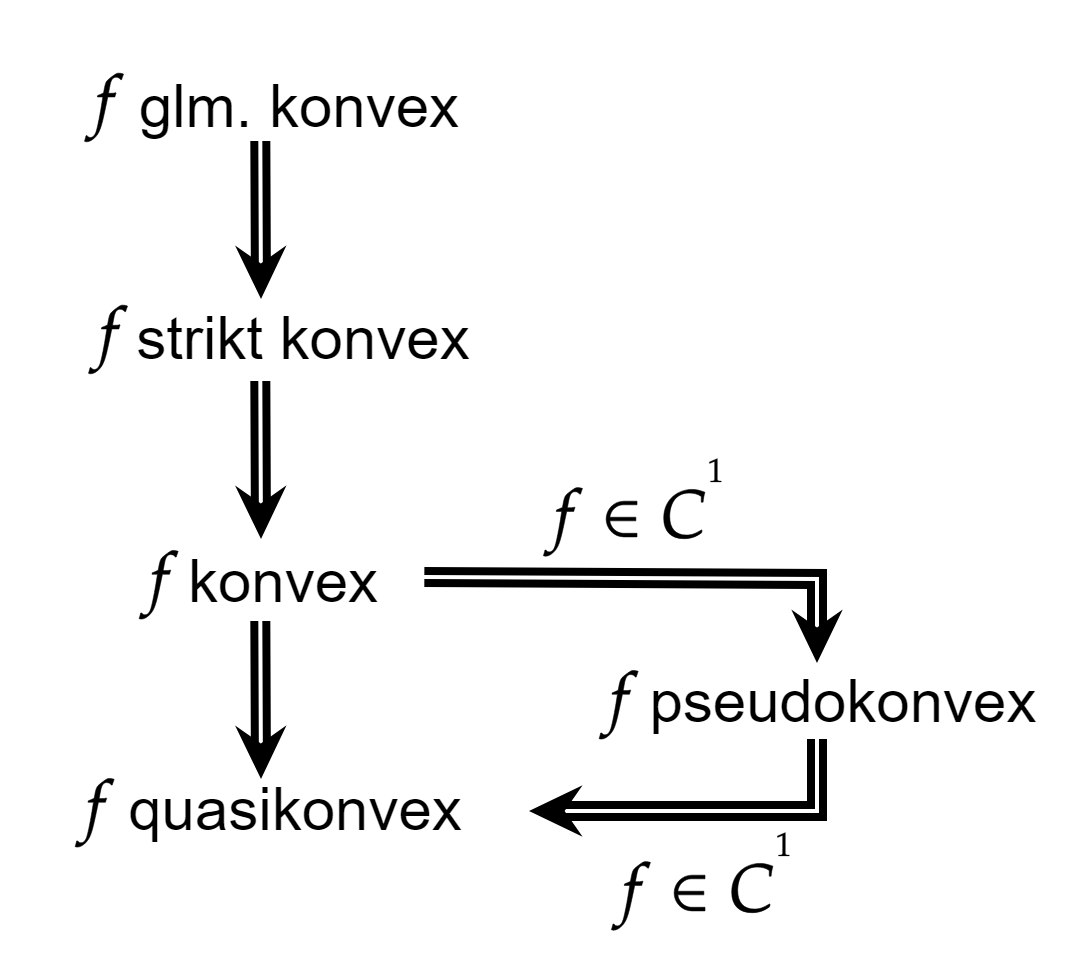
\includegraphics[width=0.5\textwidth]{pics/texplot4.png}
	\end{center}
	\caption{Übersicht über alle Arten von Konvexität und deren Zusammenhang}
	\label{fig:übersichtkonvex}
\end{figure}

